\documentclass[12pt,a4paper]{article}
\usepackage[utf8]{inputenc}
\usepackage[russian]{babel}
\usepackage[OT1]{fontenc}
\usepackage{graphicx}
\usepackage[left=1cm,right=1cm,top=1cm,bottom=1cm]{geometry}
\author{Владимир Журавлев}
\usepackage{pgfplots}
\usepackage{graphicx}
\usepackage{amsmath}
\pgfplotsset{compat=1.9}
\pagestyle{plain}
\usepackage{pgfplotstable,filecontents}

\begin{document}
\begin{flushright}

\textbf{Журавлев Владимир, 621 гр.\\}


\end{flushright}
\begin{center}
\begin{LARGE}

\vspace{\baselineskip}
Лабораторная работа №4.3.1\\
\textbf{
ИЗУЧЕНИЕ ДИФРАКЦИИ СВЕТА}\\
\vspace{\baselineskip}

\end{LARGE}
\end{center}

\subsection{A. Дифракция Френеля}

В средней волновой зоне число темных полос выражается через число зон френеля:
\[n= m - 1 \]

Рассчитаем число зон френеля для щели и построим график $2z_m = f(m)$

\begin{center}
\begin{tabular}{|c|c|c|}
\hline 
N & M & L, sm \\ 
\hline 
1 & 2 & 50.1 \\ 
\hline 
2 & 3 & 50.8 \\ 
\hline 
3 & 4 & 51.2 \\ 
\hline 
4 & 5 & 51.3 \\ 
\hline 
5 & 6 & 51.4 \\ 
\hline 
\end{tabular} 

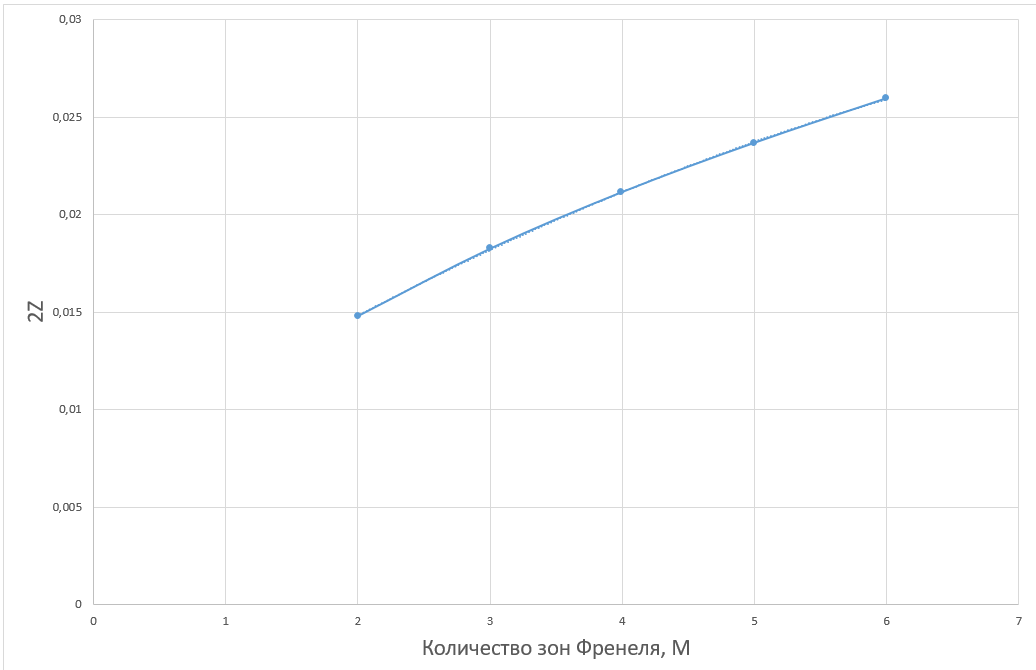
\includegraphics[scale=0.6]{451_1.png}
\end{center}
\subsection{B. Дифракция Фраунгофера}
Для дальней волновой зоны фазовые соотношения значительно упрощаются: m-ый дифракционный минимум наблюдается под таким углом, что
\[ \lambda = \delta = r_2 - r_1 = D \sin \theta\approx D\theta\]
Если мы наблюдаем дифракцию в фокальной плоскости линзы, то каждому углу соотвествует точка на расстоянии \[x = f \tan \theta\]

И для m-ого минимума:

\[X_m = f_2 m \frac{\lambda}{D} \]
\begin{center}
\begin{tabular}{|c|c|}
\hline 
m & L, 0,2 mm\\ 
\hline 
-1 & 1,8 \\ 
\hline 
0 & 3 \\ 
\hline 
1 & 4,2 \\ 
\hline 
2 & 5 \\ 
\hline 
\end{tabular} 

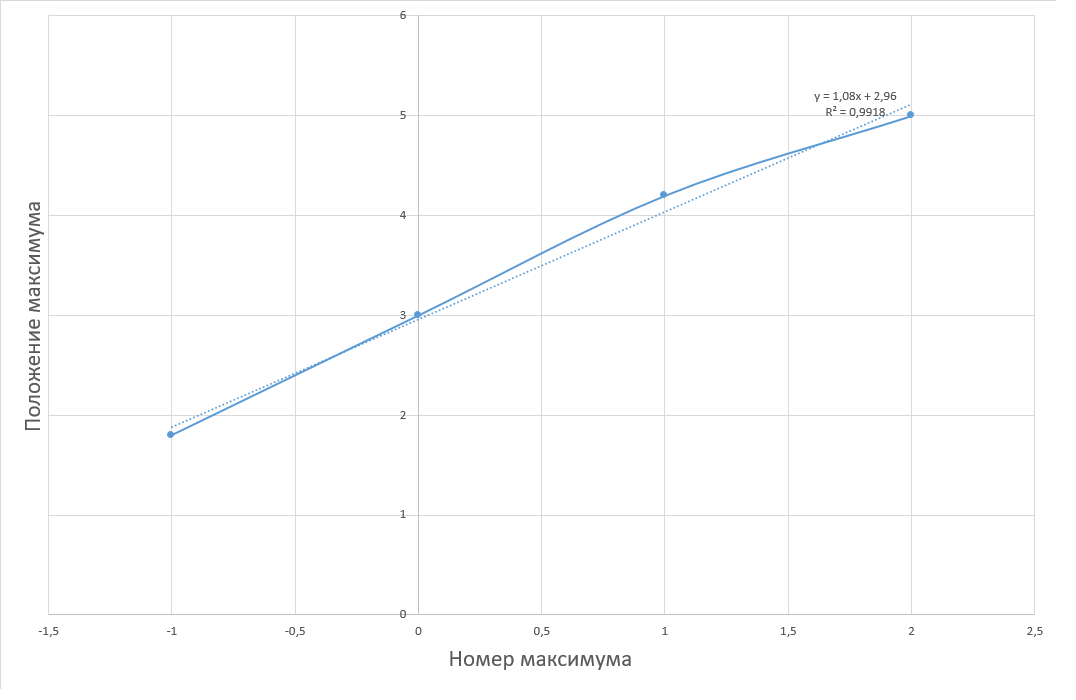
\includegraphics[scale=0.6]{451_2.png}
\end{center}
Рассчитав среднее растояние м/у минимумами можно найти ширину щели:
\[\Delta X = f_2 \frac{\lambda}{D} \Rightarrow D =  f_2 \frac{\lambda}{\Delta X } = 0.26 \; mm \pm  0.2 \; mm\]

\subsection{C. Дифракция на двух щелях}
Две щели - самая маленькая дифракционная решетка; При дифракции на двух узких щелях с расстоянием d, для дифракционных максимумов имеем:
\[d \theta = m \lambda \]
или расстояние м/у ними: $\delta = f_2 \frac{\lambda}{d}$ 
Тогда число полос в области центрального максимума
\[n = 2d/D \]
\subsection{D.Влияние дифракции на разрешающую способность прибора}
Внесем дополнительную щель для изучения влияния дифракции на ней. Ширина шели, при которой две щели неразличимы $b= 0.09 \; mm$ а $d = 35$ делений;
Расчетная ширина по критерию Релея:
\[D_0 = \frac{\lambda f_1}{l} = \frac{\lambda f_1}{d \delta} = 0.078 \pm 0.003 \; mm \]
\end{document}